\section{Reduced model and calibration framework}
\label{sec:model}

The reduced-order model used throughout this work couples a
zero-dimensional electron kinetics and power balance to a
one-dimensional radial transport equation for atomic fluorine, with
a single depletion correction linking the two. This section defines
the model, states its geometric and kinetic assumptions, and
introduces the notation used in the identifiability analysis of
Section~\ref{sec:identifiability} and subsequent sections.

\subsection{Geometry and operating conditions}
\label{sec:model:geometry}

The reactor is idealized as a right cylinder of volume $V$ operated
at a fixed chamber pressure $p$ and driven by inductive coupling at
a specified absorbed radio-frequency power $P_{\mathrm{abs}}$. The
discharge is assumed to be in steady state at each operating point,
and azimuthal and axial variations of the reactive-neutral density
are neglected. The nominal calibration condition is
$p = 10$\,mTorr and pure \sfsix{}; chamber-condition differences
between the two literature anchors are discussed in
Section~\ref{sec:baseline}.

The gas temperature at the inlet is $T_0 = 300$\,K, with a linear
power-dependent heating correction
\begin{equation}
  T_g(P_{\mathrm{abs}}) \;=\; T_0 \;+\; \alpha_T\,P_{\mathrm{abs}},
  \label{eq:gas-heating}
\end{equation}
with $\alpha_T = 0.15$\,K\,W$^{-1}$ fitted in a preliminary heating
match and held fixed in all subsequent analyses. The cold-gas
\sfsix{} density at inlet temperature is
$\nSFsix = p/(k_B T_0)$, and the F-atom diffusion coefficient
follows the hard-sphere scaling $D(T_g) = D_0(T_g/T_0)^{3/2}$.

\subsection{Electron power balance}
\label{sec:model:power}

Electron-impact rate coefficients for ionization, attachment, and
dissociative excitation of \sfsix{} are denoted
$\kiz$, $\katt$, and $\kdiss$; each is an aggregate
over the corresponding subset of processes in the Biagi
cross-section set \citep{biagi}. In Sections~\ref{sec:baseline} and
\ref{sec:identifiability}, the rate coefficients are evaluated by
convolving the cross sections with a Maxwellian distribution at the
tabulated effective electron temperature
$T_e^{\mathrm{eff}}(E/N,x_{\mathrm{Ar}})$. This rate-source choice
is revisited in Section~\ref{sec:boltzmann}.

The zero-dimensional electron-power balance equates absorbed power
to electron-energy loss through ionization and attachment:
\begin{equation}
  \nel(P_{\mathrm{abs}})
  \;=\;
  \frac{P_{\mathrm{abs}}}
       {\nSFsix\,V\,\varepsilon_{\mathrm{loss}}\,q_e},
  \qquad
  \varepsilon_{\mathrm{loss}}
  \equiv \varepsilon_{\mathrm{iz}}\kiz
         + \varepsilon_{\mathrm{att}}\katt,
  \label{eq:power-balance}
\end{equation}
with $q_e$ the elementary charge and
$\varepsilon_{\mathrm{iz}}$, $\varepsilon_{\mathrm{att}}$ the
threshold energies for the two channels. The undepleted neutral
density $\nSFsix$ enters rather than the depleted value defined
below: the electron-kinetic equilibration timescale is much shorter
than gas replenishment, so the power balance equates the
instantaneous absorbed power to the inelastic-loss flux against the
cold-gas density.

\subsection{Feedstock depletion and F-atom source}
\label{sec:model:depletion}

At high absorbed power, electron-impact dissociation becomes
comparable to gas replenishment, and the steady-state \sfsix{}
density is reduced below the inlet value. We parameterize this
effect by a single-parameter depletion correction
\begin{equation}
  n_{\mathrm{SF}_6,\mathrm{eff}}(P_{\mathrm{abs}})
  \;=\;
  \frac{\nSFsix}{1 + \beta\,\kdiss\,\nel(P_{\mathrm{abs}})},
  \label{eq:depletion}
\end{equation}
where $\beta$ is a characteristic depletion timescale with units of
seconds. Equation~\eqref{eq:depletion} is the steady-state solution
of a zero-dimensional mass balance with inflow, volumetric
dissociation loss at rate $\kdiss\nel$, and pumping loss with
timescale $\beta$. The volume-averaged atomic-fluorine source is
\begin{equation}
  \overline{S}_F(P_{\mathrm{abs}})
  \;=\;
  \nu\,\kdiss\,\nel(P_{\mathrm{abs}})\,
        n_{\mathrm{SF}_6,\mathrm{eff}}(P_{\mathrm{abs}}),
  \label{eq:source}
\end{equation}
with $\nu = 6$ the stoichiometric F atoms per dissociated \sfsix{}.

\subsection{Radial transport and etch-rate readout}
\label{sec:model:transport}

The radial F-atom density obeys a steady-state reaction--diffusion
equation in cylindrical coordinates,
\begin{equation}
  -\,\frac{1}{r}\frac{d}{dr}
  \!\left(r\,D(T_g)\,\frac{dn_F}{dr}\right)
  \;=\; S_F(r;P_{\mathrm{abs}}),
  \label{eq:transport}
\end{equation}
with a Gaussian volumetric source integrating to
$\overline{S}_F V$, and a Robin wall boundary condition
$-D\,dn_F/dr = (\gamma_{\mathrm{wall}}\vth/4)\,n_F$ at $r = R$. Since
the PDE is linear in the source amplitude, solving once with a unit
source yields a purely geometric gain factor $\mathcal{G}$ mapping
$\overline{S}_F$ to the wafer-area-averaged F density
$\langle n_F\rangle_{\mathrm{wafer}}$. The mean wafer etch rate is
\begin{equation}
  \overline{r}_{\mathrm{etch}}(P_{\mathrm{abs}})
  \;=\;
  \varepsilon\,\gamma_{\mathrm{wafer}}\,
  \frac{\vth(T_g)}{4}\,
  \langle n_F\rangle_{\mathrm{wafer}}(P_{\mathrm{abs}}),
  \label{eq:etch}
\end{equation}
with $\varepsilon$ the effective silicon removal depth per F atom
incident on the wafer (units of m\,atom$^{-1}$) and
$\gamma_{\mathrm{wafer}}$ the wafer sticking probability. The
geometric parameters
$(R,\sigma_S,\gamma_{\mathrm{wall}},\gamma_{\mathrm{wafer}})$ and
$D_0$ are held fixed; the only two parameters adjusted during
calibration are $\varepsilon$ and $\beta$.

\subsection{Calibration framework}
\label{sec:model:calibration}

Calibration proceeds in two stages. First, $\varepsilon$ is fitted
against a low-power anchor $(P_L,r_L)$ with $\beta$ held at zero.
Second, $\beta$ is introduced as a free parameter and
$(\varepsilon,\beta)$ are refitted jointly so that both anchors are
reproduced exactly. The second stage is a one-dimensional
root-finding problem in $\beta$, and no additional parameters are
adjusted. The pipeline is shown schematically in
Fig.~\ref{fig:pipeline}. Section~\ref{sec:baseline} reports the
numerical result of this procedure under the Maxwellian
rate-coefficient assumption.

\begin{figure}[t]
  \centering
  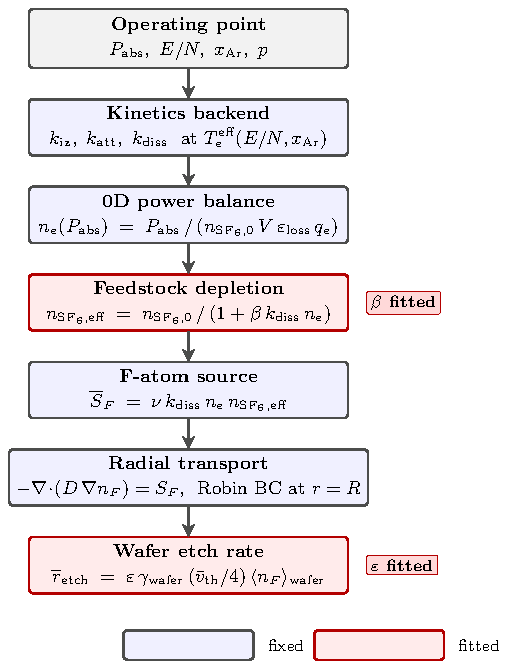
\includegraphics[width=0.85\linewidth]{figures/fig1_pipeline_schematic}
  \caption{Reduced-order \sfsix{} ICP model pipeline. Operating-point
  inputs $(P_{\mathrm{abs}},E/N,x_{\mathrm{Ar}},p)$ feed into the
  kinetics backend (Maxwellian or Boltzmann), the 0D electron power
  balance \eqref{eq:power-balance}, the feedstock-depletion
  correction \eqref{eq:depletion}, the volumetric F-atom source
  \eqref{eq:source}, the 1D radial reaction--diffusion equation
  \eqref{eq:transport}, and the wafer flux readout \eqref{eq:etch}.
  Fixed-structure blocks are shown in blue; the two fitted
  parameters $\varepsilon$ and $\beta$ are shown in red.}
  \label{fig:pipeline}
\end{figure}
